% Options for packages loaded elsewhere
\PassOptionsToPackage{unicode}{hyperref}
\PassOptionsToPackage{hyphens}{url}
\PassOptionsToPackage{dvipsnames,svgnames,x11names}{xcolor}
\documentclass[
  10pt,
  fontset=fandol]{ctexart}
\usepackage{xcolor}
\usepackage[margin=16mm]{geometry}
\usepackage{amsmath,amssymb}
\setcounter{secnumdepth}{-\maxdimen} % remove section numbering
\usepackage{iftex}
\ifPDFTeX
  \usepackage[T1]{fontenc}
  \usepackage[utf8]{inputenc}
  \usepackage{textcomp} % provide euro and other symbols
\else % if luatex or xetex
  \usepackage{unicode-math} % this also loads fontspec
  \defaultfontfeatures{Scale=MatchLowercase}
  \defaultfontfeatures[\rmfamily]{Ligatures=TeX,Scale=1}
\fi
\usepackage{lmodern}
\ifPDFTeX\else
  % xetex/luatex font selection
\fi
% Use upquote if available, for straight quotes in verbatim environments
\IfFileExists{upquote.sty}{\usepackage{upquote}}{}
\IfFileExists{microtype.sty}{% use microtype if available
  \usepackage[]{microtype}
  \UseMicrotypeSet[protrusion]{basicmath} % disable protrusion for tt fonts
}{}
\makeatletter
\@ifundefined{KOMAClassName}{% if non-KOMA class
  \IfFileExists{parskip.sty}{%
    \usepackage{parskip}
  }{% else
    \setlength{\parindent}{0pt}
    \setlength{\parskip}{6pt plus 2pt minus 1pt}}
}{% if KOMA class
  \KOMAoptions{parskip=half}}
\makeatother
\usepackage{graphicx}
\makeatletter
\newsavebox\pandoc@box
\newcommand*\pandocbounded[1]{% scales image to fit in text height/width
  \sbox\pandoc@box{#1}%
  \Gscale@div\@tempa{\textheight}{\dimexpr\ht\pandoc@box+\dp\pandoc@box\relax}%
  \Gscale@div\@tempb{\linewidth}{\wd\pandoc@box}%
  \ifdim\@tempb\p@<\@tempa\p@\let\@tempa\@tempb\fi% select the smaller of both
  \ifdim\@tempa\p@<\p@\scalebox{\@tempa}{\usebox\pandoc@box}%
  \else\usebox{\pandoc@box}%
  \fi%
}
% Set default figure placement to htbp
\def\fps@figure{htbp}
\makeatother
\setlength{\emergencystretch}{3em} % prevent overfull lines
\providecommand{\tightlist}{%
  \setlength{\itemsep}{0pt}\setlength{\parskip}{0pt}}
\usepackage{amsmath,amssymb,mathtools,needspace}
\xeCJKDeclareCharClass{CJK}{"2032,"0400->"04FF,"2160->"216B,"2460->"2473,"25A0,"25C7,"25CB,"25CF}
\IfFontExistsTF{Arial Unicode MS}{\xeCJKsetup{AutoFallBack=true}\setCJKfallbackfamilyfont{\CJKrmdefault}{Arial Unicode MS}}{}
\setcounter{secnumdepth}{0}
\setlength{\emergencystretch}{2em}
\allowdisplaybreaks
\usepackage{bookmark}
\IfFileExists{xurl.sty}{\usepackage{xurl}}{} % add URL line breaks if available
\urlstyle{same}
\hypersetup{
  pdftitle={FWT 的演化机制},
  colorlinks=true,
  linkcolor={Maroon},
  filecolor={Maroon},
  citecolor={Blue},
  urlcolor={Blue},
  pdfcreator={LaTeX via pandoc}}

\title{FWT 的演化机制}
\author{}
\date{}

\begin{document}
\maketitle

\subsubsection{10.4.2　FWT 的演化机制}\label{fwt-ux7684ux6f14ux5316ux673aux5236}

前已反复指出，二分技术是快速算法设计的基本技术。二分技术的基本点是运用某种二分手续，将所给计算问题化归为规模减半的同类问题。

对于 \(N\) 点 Walsh 变换 \(N\)-WT（10.4.1），即

\[
X(i)=\sum_{j=0}^{N-1}x(j)H_N(i,j),\quad i=0,1,\cdots,N-1.
\]

将其右端的和式对半拆开，有

\[
\begin{aligned}
X(i)&=\sum_{j=0}^{N/2-1}x(j)H_N(i,j)+\sum_{j=N/2}^{N-1}x(j)H_N(i,j)\\
&=\sum_{j=0}^{N/2-1}[x(j)H_N(i,j)+x(N/2+j)H_N(i,N/2+j)],\quad i=0,1,\cdots,N-1.
\end{aligned}
\]

然后再将这组算式对半分为两组算式，有

\[
\begin{cases}
\displaystyle X(i)=\sum_{j=0}^{N/2-1}[x(j)H_N(i,j)+x(N/2+j)H_N(i,N/2+j)],\\[6pt]
\displaystyle X(N/2+i)=\sum_{j=0}^{N/2-1}[x(j)H_N(N/2+i,j)+x(N/2+j)H_N(N/2+i,N/2+j)],
\end{cases}
\]

\[
i=0,1,\cdots,N/2-1.
\]

利用定理 1 的递推关系将上述算式化简，得

\[
\begin{cases}
\displaystyle X(i)=\sum_{j=0}^{N/2-1}[x(j)+x(N/2+j)]H_{N/2}(i,j),\\[6pt]
\displaystyle X(N/2+i)=\sum_{j=0}^{N/2-1}[x(j)-x(N/2+j)]H_{N/2}(N/2+i,j),
\end{cases}\quad i=0,1,\cdots,N/2-1.
\]

这样，所给 \(N\)-WT（10.4.1）被加工成下列两个 \(N/2\)-WT：

\[
\begin{cases}
\displaystyle X(i)=\sum_{j=0}^{N/2-1}x_1(j)H_{N/2}(i,j),\\[6pt]
\displaystyle X(N/2+i)=\sum_{j=0}^{N/2-1}x_1(N/2+j)H_{N/2}(N/2+i,j),
\end{cases}\quad i=0,1,\cdots,N/2-1.
\]

为此所要施行的二分手续是

\[
\begin{cases}
x_1(j)=x(j)+x(N/2+j),\\
x_1(N/2+j)=x(j)-x(N/2+j),
\end{cases}\quad j=0,1,\cdots,N/2-1
\tag{10.4.2}
\]

上述二分手续将所给 \(N\)-WT 加工成 2 个 \(N/2\)-WT。每个 \(N/2\)-WT 通过二分手续可进一步加工成 2 个 \(N/4\)-WT。如此反复二分，使问题的规模逐次减半，最终可将

\begin{quote}
校注（agent 补充，CH10-E001）：本页化简式及其后两个 \(N/2\)-WT 的第二式，原图均写作 \(H_{N/2}(N/2+i,j)\)，上文已照录。按前页定理 10.1 和本章对 \(N/2\) 阶矩阵的索引范围，这里的行指标 \(N/2+i\) 超出 \(0,\ldots,N/2-1\)；由 \(H_N(N/2+i,j)=H_{N/2}(i,j)\)，两处应为 \(H_{N/2}(i,j)\)。这是原书下标疑误，不是 OCR 错误。\href{../assets/ch10/erratum-p271-indices.png}{原式放大裁片}。此外，本页``定理 1''照录，所用递推关系对应前页``定理 10.1''。
\end{quote}

\href{../../source-images/pdf-272.jpeg}{原页}

\(N\)-WT 加工成 \(N\) 个 1-WT，从而得出所求的结果。这种演化过程

\[
\underset{\text{（计算模型）}}{N\text{-WT}}\Rightarrow2\text{ 个 }N/2\text{-WT}\Rightarrow4\text{ 个 }N/4\text{-WT}\Rightarrow\cdots\Rightarrow\underset{\text{（计算结果）}}{N\text{ 个 }1\text{-WT}}
\]

称作\textbf{快速 Walsh 变换}。这里箭头``\(\Rightarrow\)''表示二分手续（10.4.2）。

进一步剖析二分手续（10.4.2）的内涵，计算模型 \(N\)-WT 所要加工的数据 \(\{x(j)\}\) 是个 \(N\) 维向量，将它对半二分，得 \(N/2\) 个\textbf{平移对} \((x(j),x(N/2+j))\)。可见二分手续（10.4.2）的含义是，将平移对的两个数据相加减，因而 FWT 从属于图 10.5 的二分演化模式。

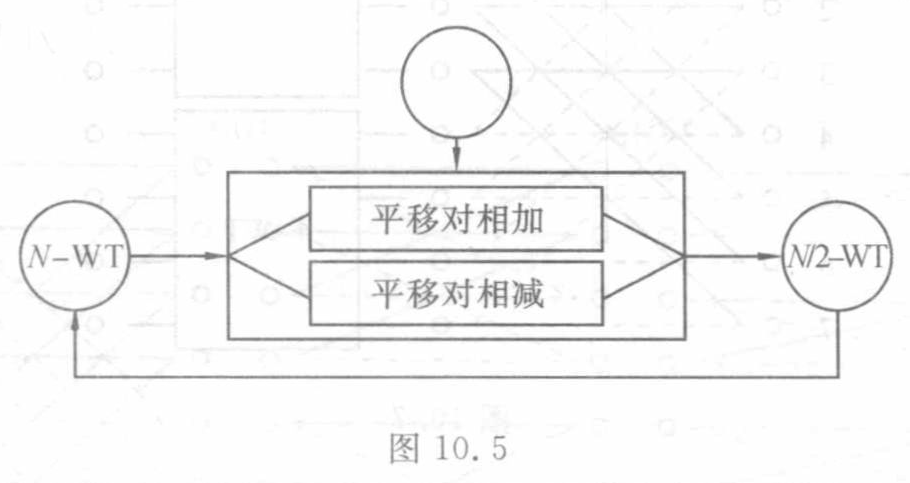
\includegraphics[width=0.85\linewidth,height=\textheight,keepaspectratio,alt={图 10.5（原图裁切）：FWT 的二分演化模式}]{../assets/ch10/fig-10-5.png}

图 10.5

\begin{quote}
图中文字与图意（转录）：左端 \(N\)-WT 进入``平移对相加''和``平移对相减''两路，合成右端 \(N/2\)-WT，底部有返回左端的反馈线；顶部有一个向下接入的空圆，原图未印文字标签。
\end{quote}

最后统计 FWT 的运算量。由于 FWT 的每一步使问题的的规模减半，欲将所给 \(N\)-WT，\(N=2^n\) 加工成 \(N\) 个 1-WT，二分演化需做 \(n=\log_2N\) 步，又形如式（10.4.2）的二分手续的每一步要做 \(N\) 次加减操作，因而 FWT 的总运算量为 \(N\log_2N\) 次加减操作。另一方面，如果直接计算 \(N\)-WT（10.4.1）要做 \(N^2\) 次加减操作，故 FWT 是快速算法，其加速比

\[
\frac{N^2}{N\log_2N}\to\infty\quad\text{（当 }N\to\infty\text{ 时）}.
\]

\begin{center}\rule{0.5\linewidth}{0.5pt}\end{center}

\subsection{相关原页校注（agent 补充）}\label{ux76f8ux5173ux539fux9875ux6821ux6ce8agent-ux8865ux5145}

以下校注来自本节覆盖的原页，可能也涉及同页相邻小节；原文照录与校正说明分开保留。

\subsubsection{原书 PDF 页 272 的校注}\label{ux539fux4e66-pdf-ux9875-272-ux7684ux6821ux6ce8}

\href{../pages/pdf-272.md}{完整原页转录} · \href{../../source-images/pdf-272.jpeg}{原页图像}

校注记录：CH10-E003。

\begin{quote}
校注（agent 补充）：原页``使问题的的规模减半''重复``的''，上文照录。
\end{quote}

\subsection{本节覆盖原页的校注记录}\label{ux672cux8282ux8986ux76d6ux539fux9875ux7684ux6821ux6ce8ux8bb0ux5f55}

下列记录按原页关联，含同页相邻小节的校注；计算时同时读取上文校注和完整原页。

\begin{itemize}
\tightlist
\item
  \texttt{CH10-E001}：原书 PDF 页 271
\item
  \texttt{CH10-E003}：原书 PDF 页 272
\end{itemize}

\end{document}
